
% Copyright (c) 2015 - 2020 Mario Mlačak, mmlacak@gmail.com
% Licensed and published as Public Domain work.

% Discovery chapter ===================================================
\chapter*{Discovery}
\addcontentsline{toc}{chapter}{Discovery}

\begin{flushright}
\parbox{0.8\textwidth}{
\emph{I don’t believe in God but I’m very interested in her. \\
\hspace*{\fill}{\textperiodcentered \textperiodcentered \textperiodcentered \hspace*{0.2em} Arthur C. Clarke} } }
\end{flushright}

\noindent
Discovery is chess variant which is played on 24 x 24 board, with
light (pastel!) yellow and gray fields and darker gray and dark teal
pieces. Star colors are bright orange and dark violet. In algebraic
notation, columns are enumerated from 'a' to 'x', and rows are
enumerated from '1' to '24'. A new piece is introduced, Monolith.

\clearpage % ..........................................................
% Monolith ************************************************************

\section*{Monolith}
\addcontentsline{toc}{section}{Monolith}

% \vspace*{-1.1\baselineskip}
\noindent
\begin{wrapfigure}[11]{l}{0.4\textwidth}
\centering
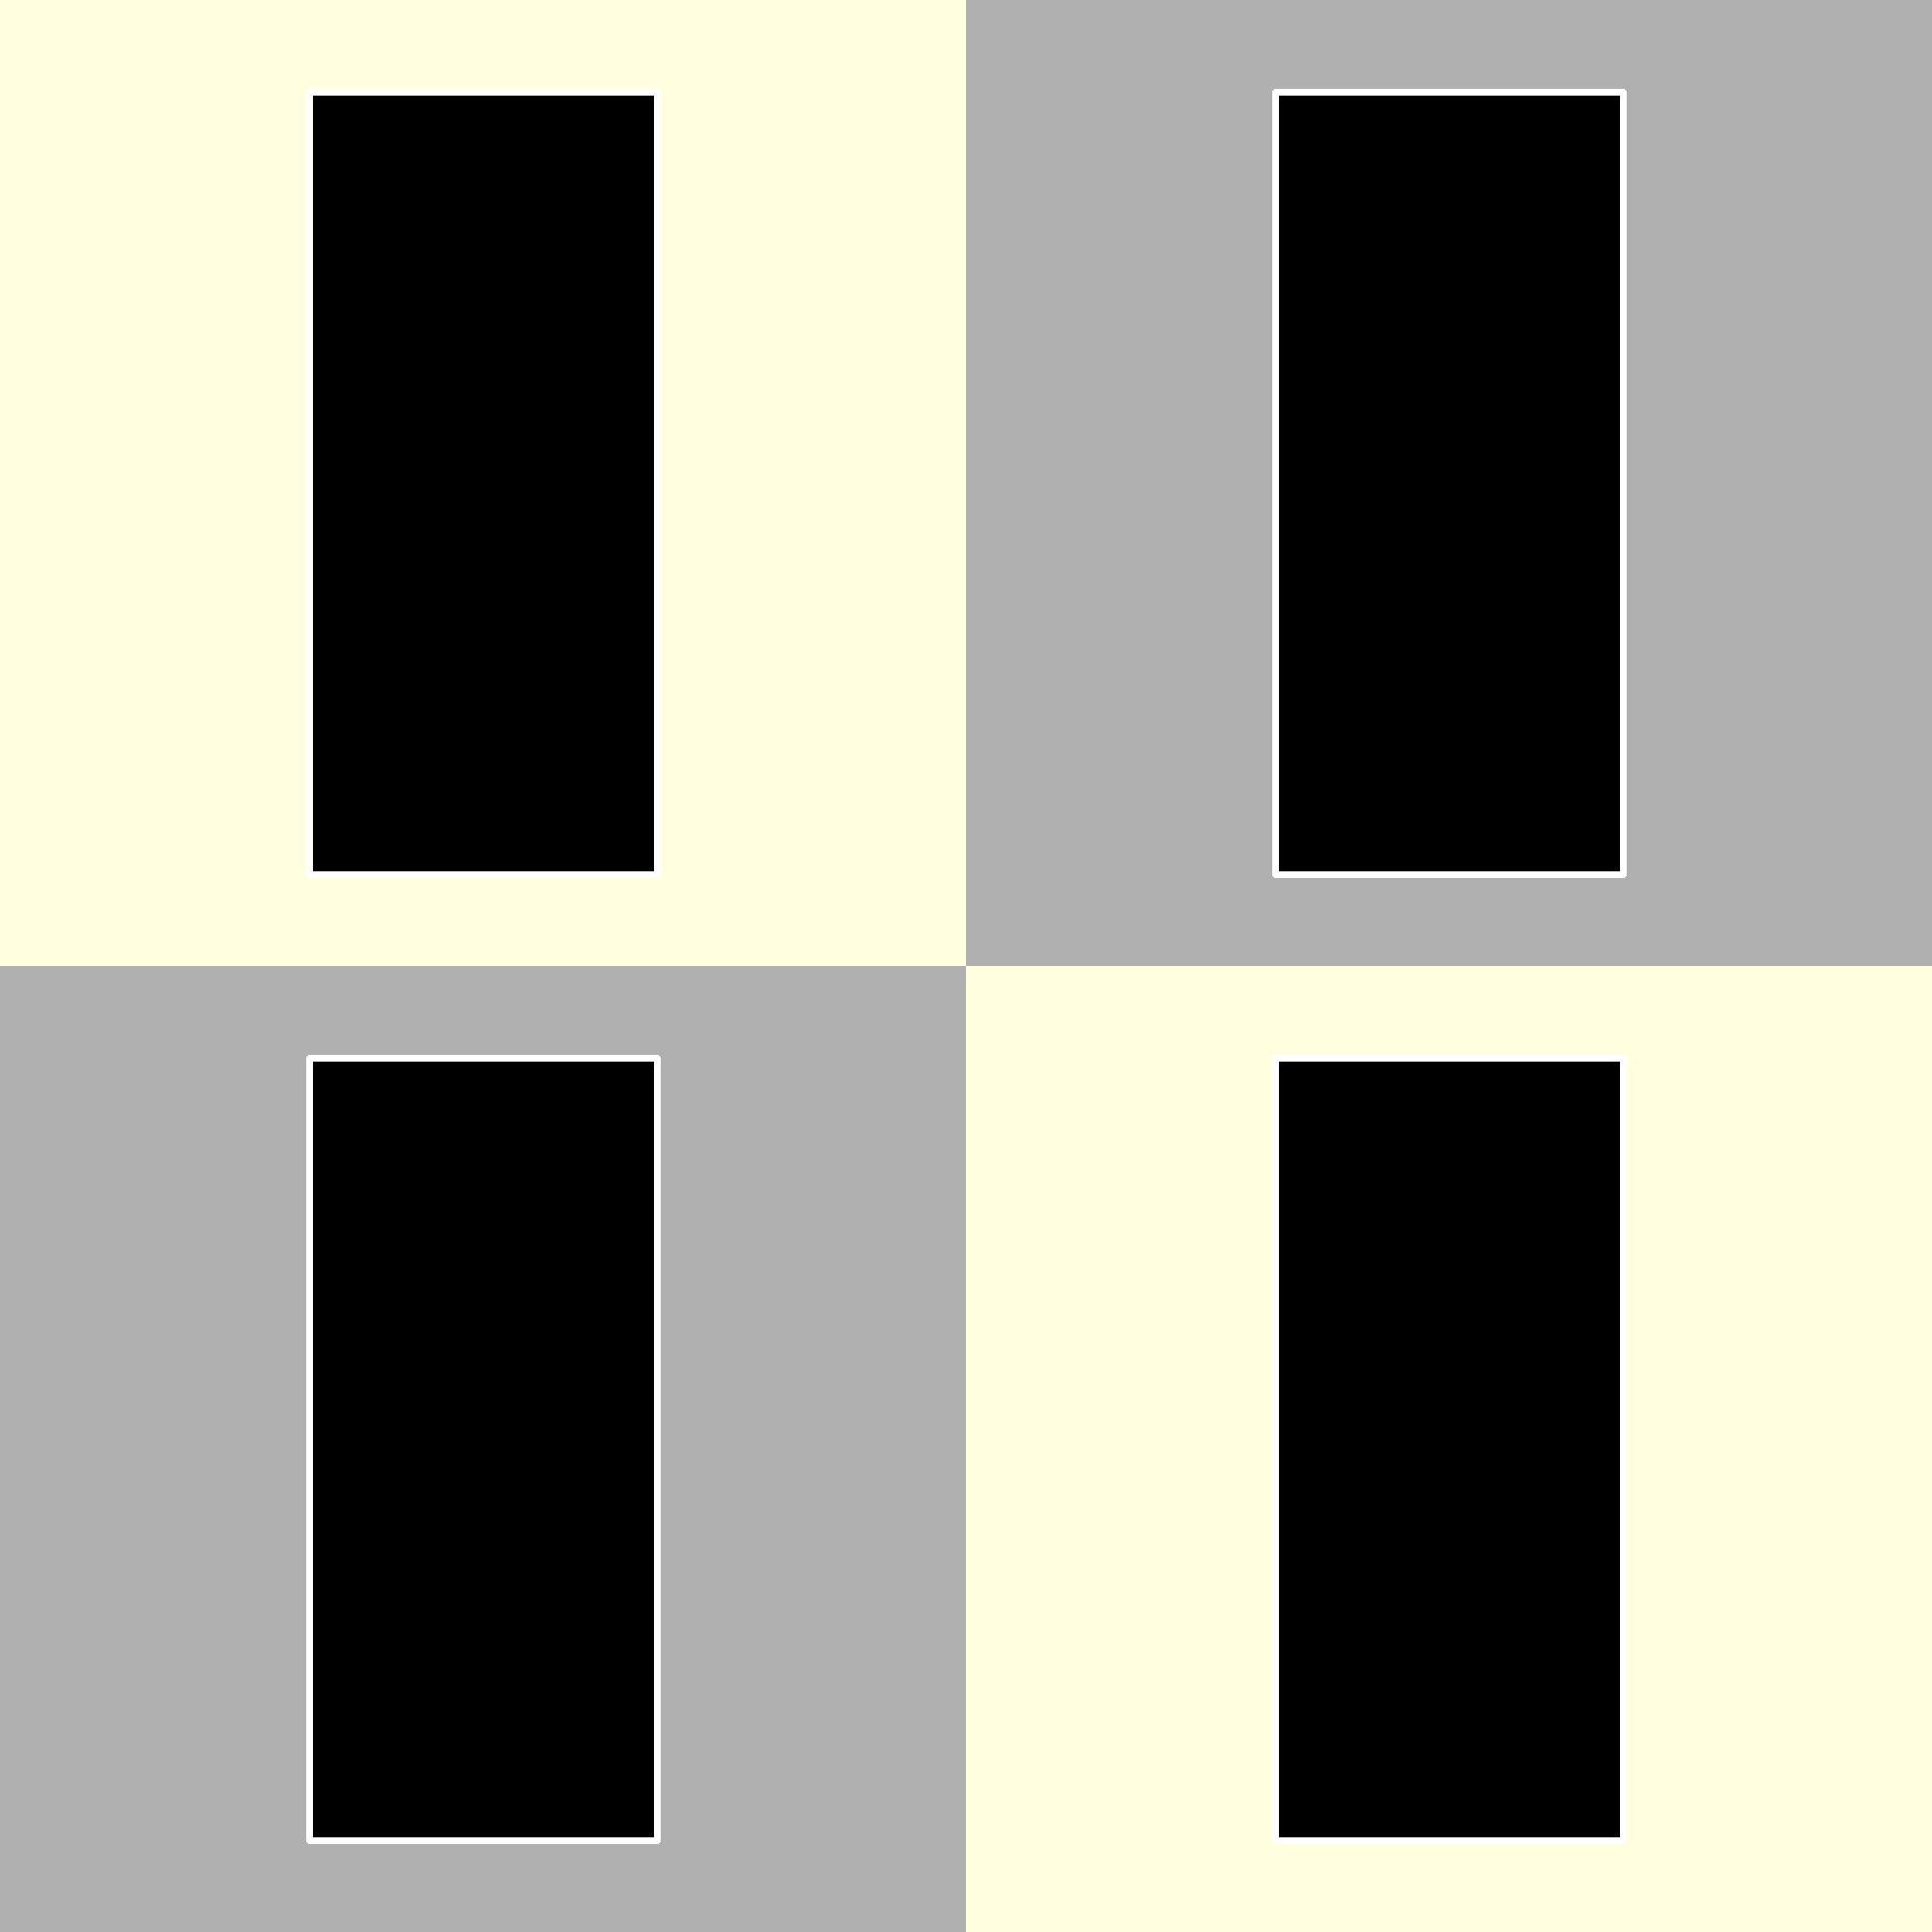
\includegraphics[width=0.4\textwidth, keepaspectratio=true]{pieces/15_monolith.png}
\caption{Monolith}
\label{fig:15_monolith}
\end{wrapfigure}
Monolith does not belong to any player, but can be moved by both of them.
Monolith cannot be captured, converted, nor activated.
Pawns cannot be promoted to Monolith.

Monolith is a teleportation device, much like moveable Star. Piece can
initiate teleportation either by touching a Monolith or a field at which
it stands.

Piece, if not Wave, then reappears on a chosen empty portal-field around
any Star or the other Monolith. Wave teleported from a Monolith can emerge
only from the other Monolith. Kings, Monoliths cannot be teleported.

Piece teleported from a Star, if not Wave, can reappear on a chosen empty
portal-field around the 2 Stars in opposite color, or around any Monolith.
Wave teleported from a Star can only emerge from the other Star in the same
color.

Monolith cannot interact with (capture, activate, ...) any piece on its own;
all step-fields in its ply must be empty. Monolith moves similar to Knight,
but can perform 3 steps in a single ply, by alternating between left and right
steps.

Alternative move for Monolith is syzygy.

In algebraic notation, symbol for Monolith is 'M'.

\clearpage % ..........................................................

% \vspace*{0.05\textheight}
\noindent
\begin{wrapfigure}[2]{l}{0.4\textwidth}
\centering
\includegraphics[width=0.4\textwidth, keepaspectratio=true]{pieces/bishop/20_discovery.png}
\caption{Bishop}
\label{fig:bishop/20_discovery}
\end{wrapfigure}
Piece colors in this variant are presented on the left.

\vspace*{0.30\textheight}
\noindent
\begin{wrapfigure}[2]{l}{0.4\textwidth}
\centering
\includegraphics[width=0.4\textwidth, keepaspectratio=true]{pieces/star/20_discovery.png}
\caption{Star}
\label{fig:star/20_discovery}
\end{wrapfigure}
Star colors in this variant are presented on the left.

\clearpage % ..........................................................
% Movement ------------------------------------------------------------

\subsection*{Movement}
\addcontentsline{toc}{subsection}{Movement}

\vspace*{-0.3\baselineskip}
\noindent
\begin{wrapfigure}[4]{l}{0.35\textwidth}
\centering
\includegraphics[width=0.291666667\textwidth, keepaspectratio=true]{examples/20_d/scn_d_01_knight_steps.png}
\caption{Knight steps}
\label{fig:scn_d_01_knight_steps}
\end{wrapfigure}
Like in a \hyperref[fig:scn_cot_10_knight_directions]{Conquest of Tlalocan variant},
looking from Knight's position forward, one direction
would be to the left, and the other to the right.

% \vspace*{0.2\textheight}
\vspace*{6.1\baselineskip}
\noindent
\begin{wrapfigure}[9]{l}{0.35\textwidth}
\centering
\includegraphics[width=0.291666667\textwidth, keepaspectratio=true]{examples/20_d/scn_d_02_monolith_steps.png}
\caption{Monolith steps}
\label{fig:scn_d_02_monolith_steps}
\end{wrapfigure}
Here, all left (green) and right (blue) steps of Monolith are marked.

Monolith can freely choose any step-field as its first step destination. On all
subsequent steps, Monolith has to alternate between left and right steps. Every
step direction can be chosen independently of any previous choice.

% \vspace*{6.1\baselineskip}
\noindent
\begin{wrapfigure}[9]{l}{0.35\textwidth}
\centering
\includegraphics[width=0.291666667\textwidth, keepaspectratio=true]{examples/20_d/scn_d_03_monolith_step_1.png}
\caption{Monolith first step}
\label{fig:scn_d_03_monolith_step_1}
\end{wrapfigure}
Like Knight, Monolith is not obstructed by any piece on unmarked (i.e. non-step)
field. Monolith cannot interact with any other piece on its own. So, Monolith is
blocked by any piece on its step-field. In this variant, Monolith is limited
to 3 steps in its ply.

\clearpage % ..........................................................

\noindent
\begin{figure}[!h]
% \begin{figure}[!t]
\includegraphics[width=1.0\textwidth, keepaspectratio=true]{examples/20_d/scn_d_04_monolith_step_2.png}
\caption{Monolith step 2}
\label{fig:scn_d_04_monolith_step_2}
% \centering
\end{figure}

Starting field is marked S. Right step was chosen as a first one, so next step
has to be to the left. Here, Monolith is obstructed by light Wave on a step-field.
This is so regardless if player moving Monolith is light or dark.

\clearpage % ..........................................................

\noindent
\begin{figure}[!h]
% \begin{figure}[!t]
\includegraphics[width=1.0\textwidth, keepaspectratio=true]{examples/20_d/scn_d_05_monolith_step_3.png}
\caption{Monolith step 3}
\label{fig:scn_d_05_monolith_step_3}
% \centering
\end{figure}

Previous step was a left one, so next step needs to be one of 4 marked right
steps. This is also last step in a Monolith's ply, since it's third. Monolith
is not obstructed by Pawns on a non-step fields; nor by Bishop on a left
step-field.

% ------------------------------------------------------------ Movement
\clearpage % ..........................................................
% Teleporting ---------------------------------------------------------

\subsection*{Teleporting}
\addcontentsline{toc}{subsection}{Teleporting}

\vspace*{-0.9\baselineskip}
\noindent
\begin{figure}[!h]
% \begin{figure}[!t]
\includegraphics[width=1.0\textwidth, keepaspectratio=true]{examples/20_d/scn_d_06_teleport_via_monolith.png}
\caption{Teleporting piece via Monolith}
\label{fig:scn_d_06_teleport_via_monolith}
% \centering
\end{figure}

Teleportation using Monoliths is similar to one using Stars in \hyperref[fig:scn_n_02_teleport_init]{previous variant, Nineteen}.
Pieces, if not Waves, teleporting from Monolith can reappear near any Star or the other Monolith.
All momentum carried is lost. Again, Kings and Monoliths cannot be teleported.
Here, all empty portal-fields where Bishop can be teleported to are enumerated.

\clearpage % ..........................................................

\noindent
\begin{figure}[!h]
% \begin{figure}[!t]
\includegraphics[width=1.0\textwidth, keepaspectratio=true]{examples/20_d/scn_d_07_teleport_via_star.png}
\caption{Teleporting piece via Star}
\label{fig:scn_d_07_teleport_via_star}
% \centering
\end{figure}

All pieces, except Waves, teleporting from a Star can reappear on a empty portal-field
near Stars in opposite color, or near any Monolith.
Here, all empty portal-fields where Bishop can be teleported to are enumerated.

\clearpage % ..........................................................
% Teleporting Wave ....................................................

\subsubsection*{Wave}
\addcontentsline{toc}{subsubsection}{Wave}

\vspace*{-1.2\baselineskip}
\noindent
\begin{figure}[!h]
% \begin{figure}[!t]
\includegraphics[width=1.0\textwidth, keepaspectratio=true]{examples/20_d/scn_d_08_teleport_wave_via_star.png}
\caption{Teleporting Wave via Star}
\label{fig:scn_d_08_teleport_wave_via_star}
% \centering
\end{figure}

Teleporting Wave using Star is the same as in \hyperref[fig:scn_n_04_teleport_move_3]{previous variant, Nineteen}.
Wave teleported from a Star emerges from the other Star in the same color,
and continues to move from position of a destination Star in the same
direction as before teleportation. Teleported Wave retains momentum carried.
Here, light Wave could activate own Bishop after teleporting with 2 momentum.

\clearpage % ..........................................................

\vspace*{-3.2\baselineskip}
\noindent
\begin{figure}[!h]
% \begin{figure}[!t]
\includegraphics[width=1.0\textwidth, keepaspectratio=true]{examples/20_d/scn_d_09_teleport_wave_via_monolith.png}
\caption{Teleporting Wave via Monolith}
\label{fig:scn_d_09_teleport_wave_via_monolith}
% \centering
\end{figure}

\vspace*{-0.3\baselineskip}
Wave teleported from a Monolith emerges from the other Monolith, and continues
movement from position of a destination Monolith in the same direction as before
teleportation, while retaining momentum carried into teleportation.
Here, light Wave could activate own Bishop after teleporting with 2 momentum.

Note, teleportation is mandatory for Wave when it reaches Monolith; Wave cannot
pass beyond it, as it can do with all the other pieces.

\clearpage % ..........................................................

\vspace*{-3.2\baselineskip}
\noindent
\begin{figure}[!h]
% \begin{figure}[!t]
\includegraphics[width=1.0\textwidth, keepaspectratio=true]{examples/20_d/scn_d_10_teleported_wave_blocked.png}
\caption{Teleported Wave blocked}
\label{fig:scn_d_10_teleported_wave_blocked}
% \centering
\end{figure}

In case where all step-fields of a teleported Wave are blocked, it is oblationed, like in
\hyperref[fig:scn_n_06_teleport_wave_blocked]{previous variant, Nineteen}.

\hyperref[fig:scn_n_03_teleport_move_2]{The same applies to all other (non-Wave) pieces}.
If all portal-fields where teleported piece could reappear are occupied, piece is removed
from chessboard.

Here, Wave cannot neither activate light Queen, nor reach any step-fields beyond Monolith;
Wave has to teleport when it reaches Monolith.

\clearpage % ..........................................................

\noindent
\begin{figure}[!h]
% \begin{figure}[!t]
\includegraphics[width=1.0\textwidth, keepaspectratio=true]{examples/20_d/scn_d_11_wave_teleported_off_board.png}
\caption{Wave teleported off-board}
\label{fig:scn_d_11_wave_teleported_off_board}
% \centering
\end{figure}

Teleported Wave with all of its step-fields located off-board is also oblationed.

\clearpage % ..........................................................

\noindent
\begin{figure}[!h]
% \begin{figure}[!t]
\includegraphics[width=1.0\textwidth, keepaspectratio=true]{examples/20_d/scn_d_12_wave_teleport_on_and_off_board.png}
\caption{Teleporting Wave on- and off-board}
\label{fig:scn_d_12_wave_teleport_on_and_off_board}
% \centering
\end{figure}

Before and after teleportation, Wave can step outside of a board, as long as its ply ends
on a board. Like in \hyperref[fig:scn_n_08_teleport_wave_end]{previous variant, Nineteen},
Wave has to continue alternating steps after teleportation; if teleported off with up-right
step, Wave has to emerge from the other Monolith with up-left step. Here, light Wave could
also activate own Bishop after teleportation with 3 momentum, or have a teleportation cascade.

\clearpage % ..........................................................

\subsubsection*{Teleportation cascade}
\addcontentsline{toc}{subsubsection}{Teleportation cascade}

\vspace*{-0.9\baselineskip}
\noindent
\begin{figure}[!h]
% \begin{figure}[!t]
\includegraphics[width=1.0\textwidth, keepaspectratio=true]{examples/20_d/scn_d_13_teleporting_wave_cascade.png}
\caption{Cascading teleportations}
\label{fig:scn_d_13_teleporting_wave_cascade}
% \centering
\end{figure}

Teleportation cascade refers to Wave being teleported at least twice in the same ply;
other pieces can't cascade teleportations. Unlike in a previous variants, thanks to
Monolith, teleportation cascade is now useful in granting access to otherwise unreachable
places. Here, light Wave can activate own Bishop only after second teleportation
(A $\rightarrow$ B, then C $\rightarrow$ D).

% .................................................... Teleporting Wave
\clearpage % ..........................................................

\subsubsection*{Trance-journey interaction}
\addcontentsline{toc}{subsubsection}{Trance-journey interaction}

\vspace*{-0.9\baselineskip}
\noindent
\begin{figure}[!h]
% \begin{figure}[!t]
\includegraphics[width=1.0\textwidth, keepaspectratio=true]{examples/20_d/scn_d_14_monolith_shaman_interaction.png}
\caption{Trance-journey interaction}
\label{fig:scn_d_14_monolith_shaman_interaction}
% \centering
\end{figure}

Like with Stars (and Kings) in \hyperref[fig:scn_cot_18_light_light_shaman_interaction_start]{the previous variant},
entranced Shamans cannot interact with Monolith, but can continue to move past it. This is so regardless of colors
of both entrancing (S) and entranced (T) Shamans. Here, entranced light Shaman can displace dark Knight, which it
can reach after passing all non-interacting pieces.

% --------------------------------------------------------- Teleporting
\clearpage % ..........................................................
% Syzygy --------------------------------------------------------------

\subsection*{Syzygy}
\addcontentsline{toc}{subsection}{Syzygy}

\vspace*{-1.2\baselineskip}
\noindent
\begin{figure}[!h]
% \begin{figure}[!t]
\includegraphics[width=1.0\textwidth, keepaspectratio=true]{examples/20_d/scn_d_15_syzygy_explain.png}
\caption{Syzygy with Stars}
\label{fig:scn_d_15_syzygy_explain}
% \centering
\end{figure}

Syzygy is alignment in one straight line of at least 3 celestial bodies, Stars and Monoliths. It's initiated by
Monolith stepping onto horizontal, vertical or diagonal line connecting 2 Stars. Syzygy-fields are all fields
where Monolith would be in syzygy. For horizontal and vertical syzygy, syzygy-fields are the same as Rook
step-fields; for diagonal syzygy, syzygy-fields are the same as Bishop step-fields.

\clearpage % ..........................................................

% \vspace*{-1.2\baselineskip}
\noindent
\begin{figure}[!h]
% \begin{figure}[!t]
\includegraphics[width=1.0\textwidth, keepaspectratio=true]{examples/20_d/scn_d_16_syzygy_2_stars_init.png}
\caption{2-Stars syzygy start}
\label{fig:scn_d_16_syzygy_2_stars_init}
% \centering
\end{figure}

Immediately after Monolith has stepped into syzygy, one own figure can then be (but don't have to be) demoted
to Pawn. Demoting to Pawn can be done even if no own Pawn has been captured yet. Opponent pieces, Kings, Stars,
Monoliths cannot be demoted. Unlike promotion, demoting to Pawn must happen in the very same move in which
Monolith has stepped into a syzygy, it cannot be saved for later.

\clearpage % ..........................................................

\noindent
\begin{figure}[!h]
% \begin{figure}[!t]
\includegraphics[width=1.0\textwidth, keepaspectratio=true]{examples/20_d/scn_d_17_syzygy_2_stars_steps.png}
\caption{2-Stars syzygy steps}
\label{fig:scn_d_17_syzygy_2_stars_steps}
% \centering
\end{figure}

If Monolith was moved into syzygy by light player, light Wave or Bishop could be demoted (blue); if moved by dark
player only dark Rook could be demoted (green). Demoting to Pawn can only be done after Monolith stepped into
alignment; once in it, no additional figures can be demoted on subsequent turns. To demote again, the same Monolith
has to step outside of alignment in one move and then back in another (or the other Monolith has to step-in).

\clearpage % ..........................................................

% \vspace*{-1.2\baselineskip}
\noindent
\begin{figure}[!h]
% \begin{figure}[!t]
\includegraphics[width=1.0\textwidth, keepaspectratio=true]{examples/20_d/scn_d_18_syzygy_2_monoliths_init.png}
\caption{2-Monoliths syzygy init}
\label{fig:scn_d_18_syzygy_2_monoliths_init}
% \centering
\end{figure}

For a Star and 2 Monoliths to be in syzygy there has to be a step which, when applied repeatedly (from a Star)
connects fields at which those celestial bodies are located. Connecting step doesn't have to correspond to the
movement of any piece, it's enough if it connects celestial bodies. Shortest such a step is called syzygy-step,
fields which are connected by syzygy-steps are called syzygy-fields. All own figures (except King) on a
syzygy-fields are then eligible to be demoted to Pawn.

\clearpage % ..........................................................

\noindent
\begin{figure}[!h]
% \begin{figure}[!t]
\includegraphics[width=1.0\textwidth, keepaspectratio=true]{examples/20_d/scn_d_19_syzygy_2_monoliths_steps.png}
\caption{2-Monoliths syzygy steps}
\label{fig:scn_d_19_syzygy_2_monoliths_steps}
% \centering
\end{figure}

Here, there is a connecting step between fields 1-3 and 3-5. There is an equivalent, shorter step connecting fields
1-2, 2-3, etc.; this is actual syzygy-step, because it is the shortest one possible. Light Knight does lay on a
syzygy-field, and so is eligible to demotion, if Monolith was moved by light player.

\clearpage % ..........................................................

\subsubsection*{Reentering syzygy}
\addcontentsline{toc}{subsubsection}{Reentering syzygy}

\vspace*{-1.2\baselineskip}
\noindent
\begin{figure}[!h]
% \begin{figure}[!t]
\includegraphics[width=1.0\textwidth, keepaspectratio=true]{examples/20_d/scn_d_20_syzygy_reentering_same_move.png}
\caption{Reentering syzygy in the same move}
\label{fig:scn_d_20_syzygy_reentering_same_move}
% \centering
\end{figure}

To be granted option to demote own figure, Monolith must move from an ordinary, non-syzygy field into syzygy. It is
not enough if Monolith in a syzygy stepped out of alignment, and then back into it, in the very same move. Monolith
which is already in a syzygy can move into the same alignment, but cannot demote any figure.

\clearpage % ..........................................................

\noindent
\begin{figure}[!h]
% \begin{figure}[!t]
\includegraphics[width=1.0\textwidth, keepaspectratio=true]{examples/20_d/scn_d_21_syzygy_reentering_independent.png}
\caption{Reentering independent syzygy}
\label{fig:scn_d_21_syzygy_reentering_independent}
% \centering
\end{figure}

The same applies even if Monolith moves into an alignment from completely independent syzygy, i.e. even if the two does
not share neither any syzygy-fields nor celestial pieces.

In short, to get option to demote again, Monolith has to move out of alignment onto an ordinary, non-syzygy field in a
first move, and then on a next move Monolith can reenter the same syzygy, or enter the other syzygy.

\clearpage % ..........................................................

\subsubsection*{In opponent's figure row}
\addcontentsline{toc}{subsubsection}{In opponent's figure row}

\vspace*{-1.2\baselineskip}
\noindent
\begin{figure}[!h]
% \begin{figure}[!t]
\includegraphics[width=1.0\textwidth, keepaspectratio=true]{examples/20_d/scn_d_22_syzygy_in_oppo_figure_row.png}
\caption{Syzygy ends with Pawn tagged for promotion}
\label{fig:scn_d_22_syzygy_in_oppo_figure_row}
% \centering
\end{figure}

Pawns which were demoted after syzygy in
\hyperref[sec:Terms/Figure row]{opponent's figure row}
are then either \hyperref[sec:Age of Aquarius/Promotion]{tagged for promotion},
or promoted straight away, in the same move, similar to
\hyperref[fig:scn_n_11_teleport_pawns_init]{previous variant, Nineteen}.

% -------------------------------------------------------------- Syzygy
% ************************************************************ Monolith
\clearpage % ..........................................................

\section*{Promotion}
\addcontentsline{toc}{section}{Promotion}

Promotion is non enforced, delayed variety, i.e. it's the same as in
\hyperref[sec:Age of Aquarius/Promotion]{previous chess variant}, Age of Aquarius.

Promotion in this variant is polygamous, more than one Queen in the same color
can be present on chessboard at any given time.

Again, Pawn cannot be promoted to Monolith.

\clearpage % ..........................................................

\section*{Rush, en passant}
\addcontentsline{toc}{section}{Rush, en passant}

\vspace*{-1.2\baselineskip}
\noindent
\begin{figure}[!h]
% \begin{figure}[!t]

\includegraphics[width=1.0\textwidth, keepaspectratio=true]{en_passants/20_discovery_en_passant.png}
\caption{En passant}
\label{fig:20_discovery_en_passant}
% \centering
\end{figure}

Rush and en passant are identical to those in \hyperref[fig:14_hemera_s_dawn_en_passant]{Hemera's Dawn variant}.
Own Pawns can be rushed for up to 10 fields in this variant.

\clearpage % ..........................................................

\section*{Castling}
\addcontentsline{toc}{section}{Castling}

Castling is the same as in Classical Chess, only difference is that King can move between 2 and 9 fields across.
All other constraints from Classical Chess still applies.

\noindent
\begin{figure}[!h]
% \begin{figure}[!t]
\includegraphics[width=1.0\textwidth, keepaspectratio=true]{castlings/20_d/discovery_castling.png}
\caption{Castling}
\label{fig:discovery_castling}
% \centering
\end{figure}

In example above, all valid King's castling moves are numbered.

\noindent
\begin{figure}[!h]
% \begin{figure}[!t]
\includegraphics[width=1.0\textwidth, keepaspectratio=true]{castlings/20_d/discovery_castling_left_07.png}
\caption{Castling long left}
\label{fig:discovery_castling_left_07}
% \centering
\end{figure}

In this example King was castling long to the left. Initial King's position is marked with "K".
After castling is finished, left Rook ends up at field immediately right to the King.

\clearpage % ..........................................................

\section*{Initial setup}
\addcontentsline{toc}{section}{Initial setup}

Compared to initial setup of Conquest of Tlalocan, just 2 Monoliths are placed in to the open,
symetrically, on both sides of chessboard. This can be seen in the image below:

\noindent
% \begin{figure}[t]
\begin{figure}[h]
\includegraphics[width=1.0\textwidth, keepaspectratio=true]{boards/20_discovery.png}
\caption{Discovery board}
\label{fig:20_discovery}
% \centering
\end{figure}

\clearpage % ..........................................................
% =================================================== Discovery chapter
